\subsection{Approximation flottante sur l'origine du point}
Afin d'éviter les auto-intersections (\textit{self-intersections}) lors de l'émission d'un nouveau rayon depuis un point d'impact, il est nécessaire de décaler légèrement son origine le long de la normale géométrique à la surface. Une approche couramment employée consiste à appliquer un décalage de longueur fixe $\varepsilon$. Cependant, cette méthode dépend de l'échelle géométrique du problème et ne garantit pas une élimination robuste des auto-intersections. Wächter et Binder \cite{Wachter2019} montrent qu'un décalage adaptatif obtenu en modifiant directement la représentation en virgule flottante des coordonnées du point d'intersection permet de produire un déplacement proportionnel à la précision numérique locale. Cette approche est ainsi pratiquement invariante vis-à-vis de l'échelle de la scène, ne nécessite aucun réglage de paramètre et limite efficacement les artefacts numériques tout en conservant un surcoût de calcul négligeable.

La Figure \ref{fig:offset} illustre le décalage potentielle entre la position calculée $p_{calc}$ et la position théorique $p_{th}$. Dans cet exemple, la position corrigée $p_{cor}$ est bien positionée par rapport à l'orientation de la surface.

Ces obversations ne sont pas présentées dans ce rapport. Mais l'approximation flottante des points d'intersection a notamment pu être mise à jour lors de rotation d'une même géométrie. Les auto-inserections pouvant atteindre $75$~\% des rayons émis sur une face. Il est important que cette correction est bien plus robuste que l'outils inhérent à la librairie \ttt{EMBREE}.

\subsection{Cas pathologique de tirage aux intersections de deux groupes}
De la même manière, un rayon peut être échantilloné sortant de la géométrie. Ce cas n'a lieu que lorsque le point est suffisamment proche d'une arrête d'un triangle, et que la frontière correspond à l'extérieur de la géométrie. La solution trouvée décale le rayon vers l'opposé la projection de la direction dans le plan d'émission (voir Figure \ref{fig:offset}). Si la situation précédente est omniprésente, celle-ci est du à un tirage de probablité faible, dans des configurations géométriques particulières. De plus, la correction est minime et ne change pas l'identité de la face récéptrice dans les conditions normales d'utilisation\footnote{La taille caratéristique du système doit être plus grande que le $\micro m$} de \ETT.
\begin{figure}[H]
\centering

\begin{minipage}{0.4\textwidth}
\centering
\vspace{3.3em}
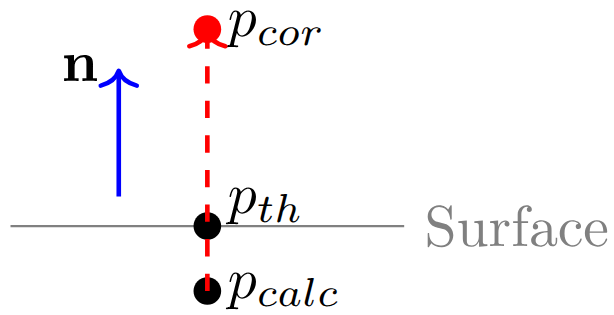
\includegraphics[width = 0.95\linewidth]{PICTURES/c2/offset_robust.png}

\small\textbf{(a) Décalage systématique}
\end{minipage}
\hfill
\begin{minipage}{0.5\textwidth}
\centering
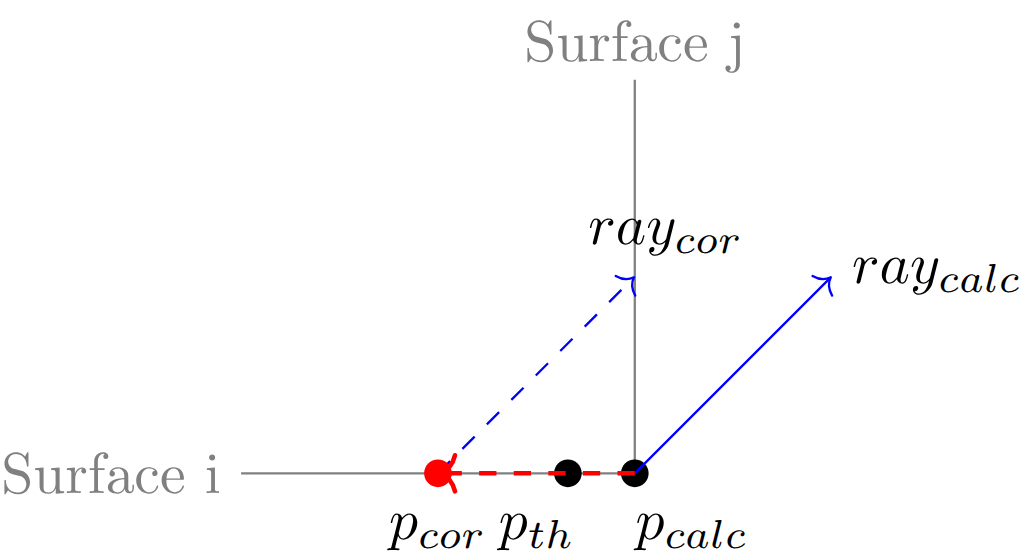
\includegraphics[width = 1\linewidth]{PICTURES/c2/offset_physic.png}

\vspace{0.3em}
\small\textbf{(b) Décalage aux arrêtes}
\end{minipage}

\caption{Illustration en 2D des décalages nécessaires pour corriger l'imprécision flottante de la position calculée .}
\label{fig:offset}

\end{figure}
\subsection{Générateur de nombre aléatoire}
expliquer brièvement pq mersen twiter + ref pour la graine.